\section{Editor}
\label{sec:editor}

\begin{figure}[htb]
    \centering
    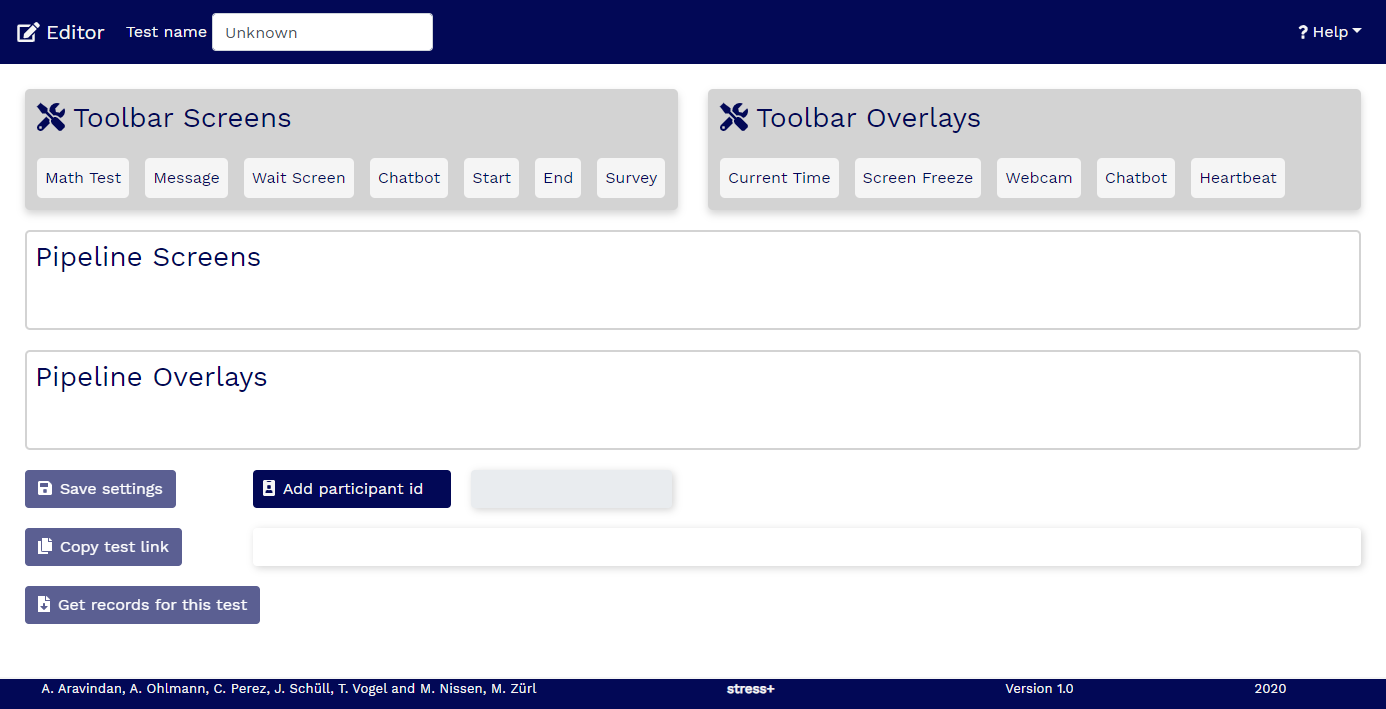
\includegraphics[width=\textwidth]{figures/screenshot-editor.png}
    \caption{Screenshot of the editor after creating a new stress test}
    \label{fig:screenshot-editor}
\end{figure}

Figure \ref{fig:screenshot-editor} shows a screenshot of the editor with an empty stress test.
With the textfield on top of the editor the name of the stress test can be changed.
All available screens and overlays are displayed in the corresponding toolbars.
From the toolbars the screen and overlay items can be moved onto the corresponding pipeline with drag and drop.
All items in the pipeline will be used when executing this stress test.
Stress test can be saved with the "Save settings" button if at least one screen item is present.
Each stress test has a unique ID that is generated when it is saved for the first time.
With this ID a link is generated that can be send to patients so they can perform the stress test.
This link is displayed next to the "Copy test link" button, which can be clicked to copy the link to the clipboard.

\begin{figure}[htb]
    \centering
    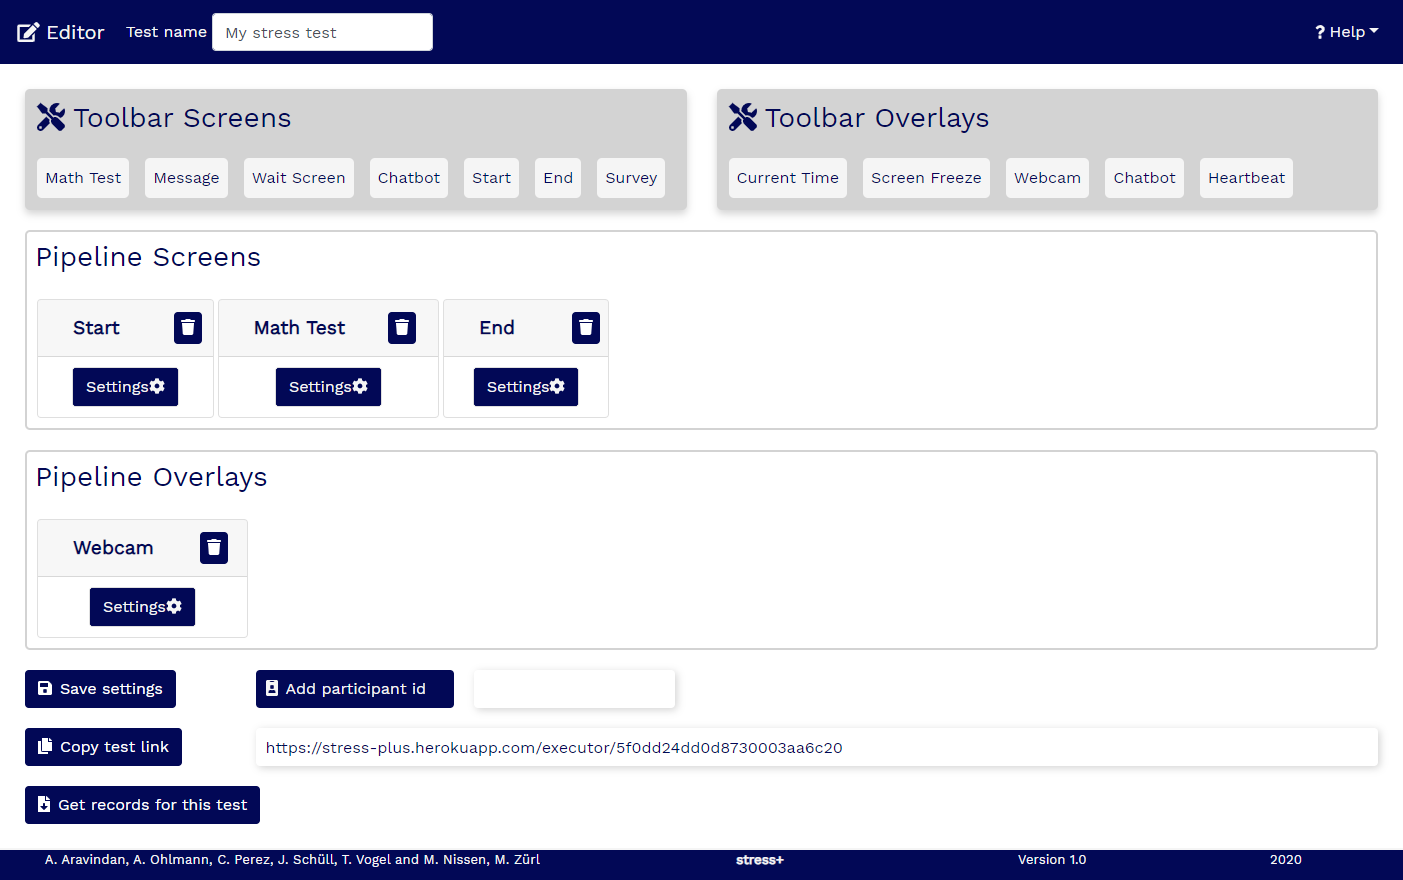
\includegraphics[width=\textwidth]{figures/screenshot-editor-with-items.png}
    \caption{Screenshot of the editor with a simple stress test}
    \label{fig:screenshot-editor-with-items}
\end{figure}

Figure \ref{fig:screenshot-editor-with-items} shows a screenshot of the editor with a simple stress test with the name "My stress test".
It consists of a "Start", "Math test" and "End" screen and uses the "Webcam" overlay.
By clicking the trash icon in the top right corner of pipeline items, the items can be deleted from the pipeline.
Each pipeline item has a "Settings" button which can be clicked to open the settings of the corresponding screen or overlay.

Clicking on the "Get records for this rest" button will download all collected test statistics of this test in JSON format.
The file will contain an array of test executions.
To differentiate test executions a participant id can be added in the textfield next to the "Add participant id" label.
This participant id will be added to the test link and to the test execution result, so executions from different participants can be identified easily.
